%Exercise 4 LaTeX report for TMA 4280
\documentclass[fontsize=11pt,paper=a4,titlepage]{report}
% \usepackage{float} %dunno yet??, probably replaced by amsfonts
\usepackage{listings}
\usepackage[usenames,dvipsnames]{color}		%For the SkyBlue background color for lstlistings
\usepackage{mathtools}
\usepackage{amsfonts,amsmath,amssymb,amsthm}	%For \mathbb
% \usepackage{caption}	%Dunno yet
\usepackage{todonotes}	%For \todo
\usepackage{tabularx}	%for tablecontents wrapping inside cell, instead of cell breaking page width.
\usepackage{verbatim}
\usepackage[margin=3cm]{geometry}

\newcommand*\Laplace{\mathop{}\!\mathbin\bigtriangleup}

\lstset{ %
language=C,							% choose the language of the code
basicstyle=\footnotesize,			% the size of the fonts that are used for the code
numbers=left,						% where to put the line-numbers
numberstyle=\footnotesize,			% the size of the fonts that are used for the line-numbers
stepnumber=1,						% the step between two line-numbers. If it is 1 each line will be numbered
numbersep=5pt,						% how far the line-numbers are from the code
backgroundcolor=\color{SkyBlue},	% choose the background color. You must add \usepackage{color}
showspaces=false,					% show spaces adding particular underscores
showstringspaces=false,				% underline spaces within strings
showtabs=false,						% show tabs within strings adding particular underscores
frame=single,						% adds a frame around the code
tabsize=4,							% sets default tabsize to 4 spaces
captionpos=b,						% sets the caption-position to bottom
breaklines=true,					% sets automatic line breaking
breakatwhitespace=false,			% sets if automatic breaks should only happen at whitespace
escapeinside={\%*}{*)}				% if you want to add a comment within your code
}

\lstset{literate=
	{á}{{\'a}}1 {é}{{\'e}}1 {í}{{\'i}}1 {ó}{{\'o}}1 {ú}{{\'u}}1
	{Á}{{\'A}}1 {É}{{\'E}}1 {Í}{{\'I}}1 {Ó}{{\'O}}1 {Ú}{{\'U}}1
	{à}{{\`a}}1 {è}{{\'e}}1 {ì}{{\`i}}1 {ò}{{\`o}}1 {ù}{{\`u}}1
	{À}{{\`A}}1 {È}{{\'E}}1 {Ì}{{\`I}}1 {Ò}{{\`O}}1 {Ù}{{\`U}}1
	{ä}{{\"a}}1 {ë}{{\"e}}1 {ï}{{\"i}}1 {ö}{{\"o}}1 {ü}{{\"u}}1
	{Ä}{{\"A}}1 {Ë}{{\"E}}1 {Ï}{{\"I}}1 {Ö}{{\"O}}1 {Ü}{{\"U}}1
	{â}{{\^a}}1 {ê}{{\^e}}1 {î}{{\^i}}1 {ô}{{\^o}}1 {û}{{\^u}}1
	{Â}{{\^A}}1 {Ê}{{\^E}}1 {Î}{{\^I}}1 {Ô}{{\^O}}1 {Û}{{\^U}}1
	{œ}{{\oe}}1 {Œ}{{\OE}}1 {æ}{{\ae}}1 {Æ}{{\AE}}1 {ß}{{\ss}}1
	{ç}{{\c c}}1 {Ç}{{\c C}}1 {ø}{{\o}}1 {å}{{\r a}}1 {Å}{{\r A}}1
	{€}{{\EUR}}1 {£}{{\pounds}}1
}
 %config.tex file in same directory

\begin{document}

\begin{center}

%\lstlistoflistings
% \listoffigures
% \listoftables

{\huge Problem set 4}\\[0.5cm]

\textsc{\LARGE TMA4280}\\[0.5cm]
\textsc{\large Introduction to supercomputing -}\\
\textsc{\large Mandatory problem set}\\[0.6cm]

\begin{table}[h]
\centering
\begin{tabular}{ccc}
	\textsc{Christian CHAVEZ}	&	\textsc{Mireia DUASO}	&	\textsc{Erlend SIGHOLT}
\end{tabular}
\end{table}

\large{\today}
\vfill
\section*{Abstract}
\end{center}

This report describes a program made to compute the sum of a Hyperharmonic
series, through a finite approximation, and comparing said sum to the known
convergence of the infinite series.

It covers the serial implementation of the summation algorithm, and exploitation
of parallelization through the OpenMP API and the Open MPI Library, in order to
improve the efficiency and speed of the program.

Finally it covers the results from utilizing parallelization, and analyzes the
utility of using parallelization to speed up this task.

\addtocounter{chapter}{1}

\clearpage
\section{Introduction}

For the programming code belonging to this problem set, see the $\textit{ex4.c}$
file in the zipped archive attached to this report. This program calculates the
difference between the sum of a finite Hyperharmonic series and the convergence
sum for an infinite Hyperharmonic series. This program is able to compute the
difference between the two in the following scenarioes listed below in
table~\ref{tab:RunModes}.

\begin{table}[h]
	\begin{tabularx}{\linewidth}{c|X|X|}
			OpenMP/MPI	& OpenMP off & OpenMP on	\\ \hline
			MPI off		& Using one thread and a single process for running the
computations serially on one processing core. & Using one process with multiple
threads on a single processing core for running the computations concurrently
across the threads. \\ \hline
			MPI on		& Using multiple processes with a single thread each,
potentially running on multiple cores concurrently for the programs
computations. & Using multiple threads in multiple processes running on
potentially multiple cores concurrently for the programs computations. \\
\hline
	\end{tabularx}
	\caption{Different runmodes for the program in this problem set.}
	\label{tab:RunModes}
\end{table}

\section{Series $S_n$}

Below (in equation~\ref{eq:HyperSeries}), the form of a~\textit{Hyperharmonic}
series is shown as

\begin{equation}
	\sum_{i=1}^{\infty} \frac{1}{i^p}.
	\label{eq:HyperSeries}
\end{equation}

However, this problem set only asks for the sum of a certain subset of
Hyperharmonic series, when $p = 2$. Below (in equation~\ref{eq:HyperSum}), the
$n$th partial sum follows the form

\begin{equation}
	S_n = \sum_{i=1}^{n} \frac{1}{i^2}.
	\label{eq:HyperSum}
\end{equation}

This problem set asks for a program that can calculate the sum of Hyperharmonic
series of the form shown in equation~\ref{eq:HyperSeries}, of finite length $n$
as shown in equation~\ref{eq:HyperSum}.

Since the problem set wants us to develop a program which can concurrently
calculate this sum in parallel on $P = 2^m$ discrete processors, this problem
set also specifies that $n$ should follow certain conditions; $n = 2^k$, where
$k$ is given as parameter on the form $\{k \in \mathbb{N} : k \in [3, 14]\}$.

The sum the problem set wants us to find the difference from, is

\begin{equation}
	\frac{\pi^2}{6} = \lim_{n \to \infty}S_n = \sum_{i=1}^{\infty} \frac{1}{i^2}.
	\label{eq:HyperActualSum}
\end{equation}

It is the difference between this sum and the $n$th partial sum of Hyperharmonic
series the problem set is interested in, and our program can calculate both
serially and in parallel.

\section{Concurrency Implementation}

The program was developed in iterations. The first iteration ran on a single
thread in a single process, in a non-concurrent sequential fashion. The second
iteration introduced running the program as mentioned in the top-right cell of
table~\ref{tab:RunModes}. This was enabled by putting the following line into
our \textit{ex4.c} file.

\lstinputlisting[firstline=18,lastline=18,firstnumber=18,label=lst:OpenMP]{
../ex4.c}

The third iteration focused on enabling the program to run in the runmode
corresponding to the bottom-right cell of table~\ref{tab:RunModes}. Since OpenMP
is enabled through the use of pragmas, making the code run with MPI alone is
then only a matter of choosing the right compiler and compilation switches.
Hence, in effect the third iteration only focused on implementing MPI into the
program.

To utilize MPI, the program does need to use a subset of the available MPI
function calls; $\textit{MPI\_Scatter()}$, $\textit{MPI\_Send()}$,
$\textit{MPI\_Reduce()}$, $\textit{MPI\_Gather()}$, $\textit{MPI\_Init()}$,
$\textit{MPI\_Finalize()}$, and so on. Not all of these are necessary, but a
minimum subset of these are. Such as, $\textit{MPI\_Init()}$ and $\textit{
MPI\_Finalize()}$, and then one of the $\textit{MPI\_Scatter()}$ or
$\textit{MPI\_Send()}$ alternatives to send data among the processes used by
MPI. Likewise there are multiple alternatives for $\textit{MPI\_Gather()}$ and
$\textit{MPI\_Reduce()}$, but you only need one of the alternatives to receive
data from the other processes used by MPI.

In our solution, found in the attached code, we utilized the following MPI
functions:

\begin{itemize}
	\item{$\textit{MPI\_Init()}$ and $\textit{
MPI\_Finalize()}$ through the provided \textit{common.c} \textit{common.h}
framework.}
	\item{$\textit{MPI\_Scatter()}$ and $\textit{MPI\_Reduce()}$ were used to
distribute 	and gather data respectively, and $\textit{MPI\_Reduce()}$ also
aided us by performing the summing necessary between the processes for us,
storing the result in a specified variable.}
\end{itemize}

These function calls are considered more convenient considering the purpose of
this problem set. This due to the fact that the problem is relatively simple,
and easy to load-balance. Hence, no complicated send/receive inter-communication
between the processes is needed to coordinate the concurrency. All the summing
is done independently of any other sum (besides the final summation performed by
$\textit{MPI\_Reduce()}$).

MPI could also have been utilized through the use of the $\textit{MPI\_Send()}$
and/or $\textit{MPI\_Gather()}$ functions. This would have provided more
detailed control over the data (-location and -communication), but this is not
necessary for solving this problem. And might in fact harm the efficiency. This
is due to potential added overhead for communication and variable assignment.
(This assumes that the library implementation of $\textit{MPI\_Reduce()}$ is
more efficient than any manual summing through the use of Send/Gather would be).

\section{Program Load}

\subsection{Memory requirement}
\label{subsec:MemReq}

The program developed for this problem set requires a certain amount of
available memory to run. There are several factors and variables to take into
account, which can all differ according to the runmodes of the program (level of
parallelism or lack thereof) and circumstance.

Since the problem set specifies the circumstance $n \gg 1$, we will ignore the
negligible extra memory needed for OpenMP. This is because a set of threads
managed by OpenMP, specifically performing a summation (as shown in
subsection~\ref{lst:OpenMP}), will have an insignificant impact on the programs
memory usage.

Hence, below there are two equations where we detail how we believe the \textit{
non-negligible} memory requirement should behave when run in a single process,
or in $P$ processes with input size decided by variable $k$ as a deciding factor
in either case.

\begin{equation}
	noMPImem = supVars\footnote{supVars = support Variables. This amount is
static, and very negligible compared to the sum describing the size of the
vector.} + \sum_{i=1}^{2^k}
sizeof(double)
	\label{eq:noMPI-Mem}
\end{equation}

\begin{equation}
	MPImem = noMPImem + (P-1)\footnote{P = $2^m$ = amount of processes the
program is run on concurrently though MPI.} \cdot supVars + P \cdot
\sum_{i=1}^{2^{k-m}} sizeof(double)
	\label{eq:MPI-Mem}
\end{equation}

As detailed above in equation~\ref{eq:MPI-Mem} (parallel circumstance), you can
see that the memory requirement ``noMPImem'' detailed in
equation~\ref{eq:noMPI-Mem} (serial circumstance), will always be present.
However, the sum term in equation~\ref{eq:MPI-Mem} can be thought of as a
duplication of the sum representing the memory required for the length of the
vector representing the Hyperharmonic series in equation~\ref{eq:noMPI-Mem}.

The only difference being that its memory requirement is spread across the $P$
processes.

\subsection{Mathematical computation}

The computational load (mathematical complexity) of our program can be given as
the amount of \textit{\textbf{Fl}oating-point \textbf{Op}erations} (FLOPs) it
needs to complete for a given input. Since this program computes the sum of a
Hyperharmonic finite series, below we detail the math describing the amount of
FLOPs behind the programs computations.

The mathematical operation needed to generate each term of the Hyperharmonic
series is as follows;

\begin{equation}
	v_i = \frac{1}{i^2}.
\end{equation}

Analyzing how many FLOPs are required for generating a term $v_i$, we see that
it requires a multiplication ($i\cdot i = i^2 = X$) and a division
($\frac{1}{X}$). A total of 2 FLOPs. So to generate a Hyperharmonic series of
$n$ terms, requires $2n$ FLOPs. In equation~\ref{eq:HyperSum} the formula the
program used for calculating the sum of the finite length Hyperharmonic series
is detailed.

The total amount of FLOPs needed for computing a Hyperharmonic series of length
$n$ will then be $2n + n = 3n$. Thus, as we have used $k$ to define the length
of $n$, $n=2^k$, the computational cost of our program can be described as;
$2^k\cdot 3$ FLOPs.

\subsection{Load-balancing}

The program developed is very well load-balanced for this specific problem set.
The problem set specifies the length of the vectors (representing the
Hyperharmonic series) to be $2^k$ long, and that our MPI implementation should
only run on a system using $P$ processors where $P$ is a power of 2.

It should be mentioned that the program does some pre-processing serially,
mandated by the task and by MPI. The initialization is necessary and
unavoidable, and the generation of the vector would probably not benefit much
(if at all) by parallelization, as the current implementation of the program stands.

However, if the problem set did not specify that rank 0 has to generate the
vector representing the Hyperharmonic series, there is both time and space to be
saved if each rank generated and  summed each its own parts of the vector. Since
that is not the case, and it is mandatory in this problem set for rank 0 to
generate the vector, the potential gain in both memory space would be

\begin{equation}
	mem\_req = \frac {current\_mem\_req}{2}.
	\label{eq:mem-req}
\end{equation}

And the gain in processing time would be

\begin{equation}
	time\_spent\_generating\_vector = \frac
{original\_time\_spent\_generating\_vector}{max(rank)+1}.
	\label{eq:time-req}
\end{equation}

Either way, the computations involved in the initialization of the
problem will be insignificant compared to the overall runtime for problem sizes
of any considerable size\footnote{$n \gg 1$, as referenced in
subsection~\ref{subsec:MemReq}.}. This stands equally true for the initial
generation of the vector representing the Hyperharmonic series of the problem
set.

Hence, the summation cost of the double-values in the vector of length $2^k$ can
always be divided equally among $P = 2^m$ processors, as long as $k\geq m$. The
parallelism is possible due to the fact that all partial sums are completely
independent of each other.

Therefore, we are convinced that you can safely conclude that within the
parameters given in this problem set, this problem is very attractive to solve
through parallel processing.

\section{Results}

\subsection{General about results}
When testing the results on kongull we had issues with the jobs not progressing fast enough in the queue, and consequently we received little usable data in time for the assignment.
To somewhat make up for this lack, some data was run on a local machine; a laptop with Ubuntu. This machine, however, only had 2 physical cores, which hampered the testing a lot. During this testing some improvement was shown, but not very much, possibly due to only 2 cores being utilized.

\subsection{Local testing}
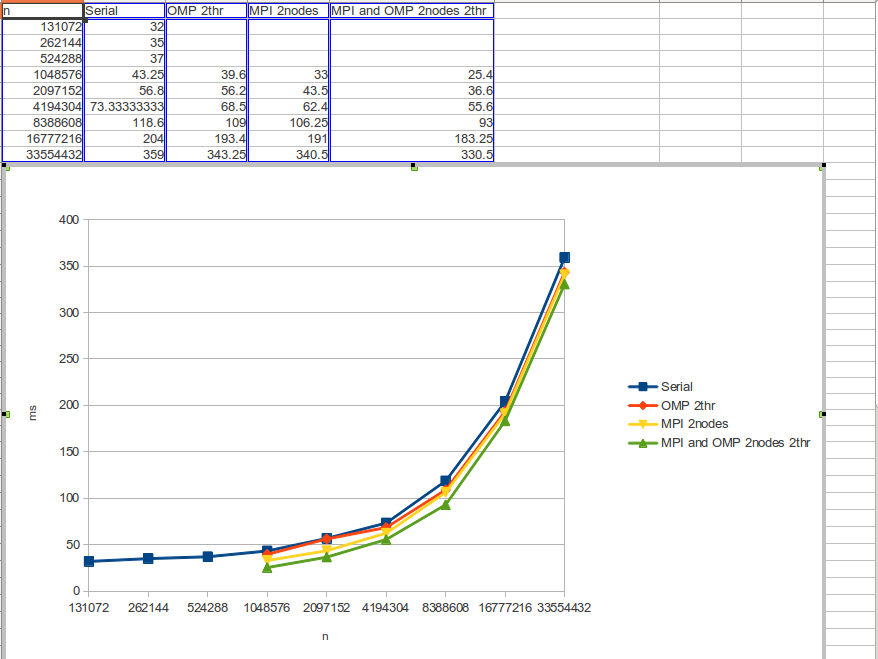
\includegraphics[scale=0.6]{local_data_plot.png}
Plot of testing locally, that shows improvement, though not to a very large degree, when utilizing parallelisation on 2 cores.

\subsection{Serial implementation}
The serial implementation increases about linearily with respect to the input size n, which indicates that
the algorithm is sufficiently efficient to use as a base for parallelization.

\subsection{OpenMP implementation}

\subsection{MPI implementation}
The local testing showed that this had a larger impact on performance than OpenMP, which indicates that doing partial summing, with the final summing done by the Reduce function is more efficient than plain speeding up summing.

\subsection{MPI + OpenMP implementation}
The plot showed that a combination of the two parallelization techniques shows the best improvement

\subsection{Combined implementation}

\end{document}
